\documentclass[aspectratio=43]{beamer}

\usepackage{amsmath}
\usepackage{amsfonts}
\usepackage{amssymb}
\usepackage{amsthm}
\usepackage{tikz}
\usepackage{xcolor}
\usepackage{array}
\usepackage{enumitem}
\usepackage{tabularx}

\usetheme{Madrid}
\usecolortheme{default}

\setbeamertemplate{navigation symbols}{}

\setbeamertemplate{footline}{}

\title{}
\author{}
\date{}

\begin{document}
\begin{frame}
\frametitle{Counting ordered rooted trees}
\end{frame}

\begin{frame}
\begin{itemize}
    \item[] \textbf{Theorem}
    \item[] The number of ordered rooted trees on $n+1$ unlabeled vertices is $C_n$.
\end{itemize}
\begin{center}
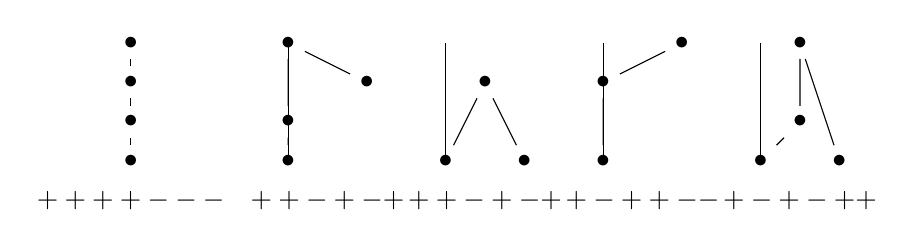
\begin{tikzpicture}
    \node (a) at (0,0) {$\bullet$};
    \node (b) at (0,0.5) {$\bullet$};
    \node (c) at (0,1.0) {$\bullet$};
    \node (d) at (0,1.5) {$\bullet$};
    \draw (a) -- (b) -- (c) -- (d);
    \node at (0,-0.5) {$++++---$};

    \draw (2,0) -- (2,1.5);
    \node (a2) at (2,0) {$\bullet$};
    \node (b2) at (2,0.5) {$\bullet$};
    \node (c2) at (2,1.5) {$\bullet$};
    \node (d2) at (3,1) {$\bullet$};
    \draw (a2) -- (b2) -- (c2) -- (d2);
    \node at (2.5,-0.5) {$++-+-+$};

    \draw (4,0) -- (4,1.5);
    \node (a3) at (4,0) {$\bullet$};
    \node (b3) at (5,0) {$\bullet$};
    \node (c3) at (4.5,1) {$\bullet$};
    \draw (a3) -- (c3) -- (b3);
    \node at (4.5,-0.5) {$++-+-+$};

    \draw (6,0) -- (6,1.5);
    \node (a4) at (6,0) {$\bullet$};
    \node (b4) at (6,1) {$\bullet$};
    \node (c4) at (7,1.5) {$\bullet$};
    \draw (a4) -- (b4) -- (c4);
    \node at (6.5,-0.5) {$+-++--$};

    \draw (8,0) -- (8,1.5);
    \node (a5) at (8,0) {$\bullet$};
    \node (b5) at (9,0) {$\bullet$};
    \node (c5) at (8.5,1.5) {$\bullet$};
    \node (d5) at (8.5,0.5) {$\bullet$};
    \draw (a5) -- (d5) -- (c5) -- (b5);
    \node at (8.5,-0.5) {$+-+-++$};

\end{tikzpicture}
\end{center}
\end{frame}

\begin{frame}
\begin{itemize}
    \item[] \textbf{Proof}
    \item[] The claim will follow once we establish a bijection between ordered rooted trees on $n+1$ vertices and ballot sequences of length $2n$.
    \item[] To construct such a bijection, trace the outer boundary of a tree, recording each step down as a $+$, and each step up as a $-$.
\end{itemize}
\end{frame}

\begin{frame}
\frametitle{Counting ordered rooted trees}

\begin{block}{Theorem}
The number of ordered rooted trees on $n+1$ unlabeled vertices is $C_n$.

\centering
\begin{tabular}{ccccc}
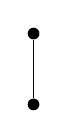
\begin{tikzpicture}[scale=0.3]
\node (root) at (0,0) [circle,fill,inner sep=1.5pt] {};
\node (child1) at (0,3) [circle,fill,inner sep=1.5pt] {};
\draw (root) -- (child1);
\end{tikzpicture}
&

\begin{tikzpicture}[scale=0.3]
\node (root) at (0,0) [circle,fill,inner sep=1.5pt] {};
\node (child1) at (-1,2) [circle,fill,inner sep=1.5pt] {};
\node (child2) at (1,2) [circle,fill,inner sep=1.5pt] {};
\draw (root) -- (child1);
\draw (root) -- (child2);
\end{tikzpicture}
&
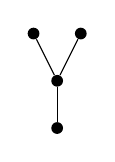
\begin{tikzpicture}[scale=0.3]
\node (root) at (0,0) [circle,fill,inner sep=1.5pt] {};
\node (child1) at (0,2) [circle,fill,inner sep=1.5pt] {};
\node (child2) at (-1,4) [circle,fill,inner sep=1.5pt] {};
\node (child3) at (1,4) [circle,fill,inner sep=1.5pt] {};
\draw (root) -- (child1);
\draw (child1) -- (child2);
\draw (child1) -- (child3);
\end{tikzpicture}
&
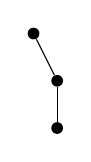
\begin{tikzpicture}[scale=0.3]
\node (root) at (0,0) [circle,fill,inner sep=1.5pt] {};
\node (child1) at (0,2) [circle,fill,inner sep=1.5pt] {};
\node (child2) at (-1,4) [circle,fill,inner sep=1.5pt] {};
\draw (root) -- (child1);
\draw (child1) -- (child2);
\end{tikzpicture}
&
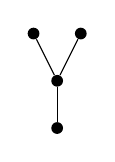
\begin{tikzpicture}[scale=0.3]
\node (root) at (0,0) [circle,fill,inner sep=1.5pt] {};
\node (child1) at (0,2) [circle,fill,inner sep=1.5pt] {};
\node (child2) at (-1,4) [circle,fill,inner sep=1.5pt] {};
\node (child3) at (1,4) [circle,fill,inner sep=1.5pt] {};
\draw (root) -- (child1);
\draw (child1) -- (child2);
\draw (child1) -- (child3);
\end{tikzpicture}
\\
$+++\,--$ & $++--+$ & $++-+--$ & $+--++-$ & $+-+-++$
\end{tabular}
\end{block}

\begin{block}{Proof}
The claim will follow once we establish a bijection between ordered rooted trees on $n+1$ vertices and ballot sequences of length $2n$.
To construct such a bijection, trace the outer boundary of a tree, recording each step down as a $+$, and each step up as a $-$.
\end{block}

\begin{block}{Exercise}
Draw the tree corresponding to $++--+--++--+--$
\end{block}

\end{frame}

\begin{frame}
\frametitle{Rooted trees}

\begin{block}{Definition}
A \alert{rooted tree} $T$ is a finite set of elements (called \alert{vertices}) together with an additional structure of \alert{parent-child} binary relation on $T$. This relation must satisfy the following requirements:
\begin{itemize}
    \item there is a distinguished \alert{root} vertex without a parent;
    \item each non-root vertex has a unique parent;
    \item each vertex is a descendent of the root.
\end{itemize}
\end{block}

\begin{block}{Pictorial representation}
    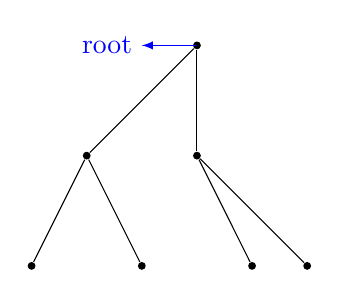
\begin{tikzpicture}[scale=0.7]
    \node[circle, fill=black, inner sep=1pt] (r) at (0,0) {};
    \node[circle, fill=black, inner sep=1pt] (a) at (-2,-2) {};
    \node[circle, fill=black, inner sep=1pt] (b) at (0,-2) {};
    \node[circle, fill=black, inner sep=1pt] (c) at (-3,-4) {};
    \node[circle, fill=black, inner sep=1pt] (d) at (-1,-4) {};
    \node[circle, fill=black, inner sep=1pt] (e) at (1,-4) {};
    \node[circle, fill=black, inner sep=1pt] (f) at (2,-4) {};
    
    \draw (r) -- (a);
    \draw (r) -- (b);
    \draw (a) -- (c);
    \draw (a) -- (d);
    \draw (b) -- (e);
    \draw (b) -- (f);
    
    \draw[blue, -latex] (0,0) -- (-1,0) node[anchor=east, blue]{root};
    \end{tikzpicture}
\end{block}

\end{frame}

\begin{frame}
\frametitle{Examples of rooted trees}

\begin{itemize}
    \item genealogical trees
    \item evolutionary trees
    \item organizational charts
    \item subordination hierarchies
    \item taxonomy hierarchies
    \item administrative geography
    \item playoff brackets
    \item decision trees
    \item hierarchical file systems
    \item search/sorting trees
    \item parse/syntax trees
    \item recursion trees
\end{itemize}

\end{frame}

\begin{frame}
\frametitle{Ordered rooted trees}

\begin{block}{Definition}
A rooted tree is called \textcolor{blue}{ordered} if it is endowed with a prescribed linear
ordering (``left to right'') among the children of each internal vertex.
\end{block}

\begin{block}{Example}
Rules of succession or inheritance based on primogeniture.

The ordering of a rooted tree can be encoded by a \textcolor{blue}{planar embedding}.

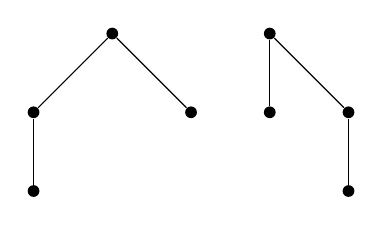
\begin{tikzpicture}
  \node[circle, fill=black, inner sep=1.5pt] (a) at (0,0) {};
  \node[circle, fill=black, inner sep=1.5pt] (b) at (0,1) {};
  \node[circle, fill=black, inner sep=1.5pt] (c) at (1,2) {};
  \node[circle, fill=black, inner sep=1.5pt] (d) at (2,1) {};

  \draw (a) -- (b);
  \draw (b) -- (c);
  \draw (c) -- (d);

  \node[circle, fill=black, inner sep=1.5pt] (a2) at (4,0) {};
  \node[circle, fill=black, inner sep=1.5pt] (b2) at (4,1) {};
  \node[circle, fill=black, inner sep=1.5pt] (c2) at (3,2) {};
  \node[circle, fill=black, inner sep=1.5pt] (d2) at (3,1) {};

  \draw (a2) -- (b2);
  \draw (b2) -- (c2);
  \draw (c2) -- (d2);

\end{tikzpicture}

\end{block}

\end{frame}

\begin{frame}
\frametitle{Rooted trees as graphs}

Rooted trees are examples of \textcolor{blue}{graphs}. We shall study graphs
systematically in the second half of the course.

\begin{block}{Definition}
A vertex with no children is called a \textcolor{blue}{leaf}. The remaining vertices are
called \textcolor{red}{internal}. A parent-child pair in a rooted tree forms an \textcolor{blue}{edge}.
\end{block}

\begin{center}
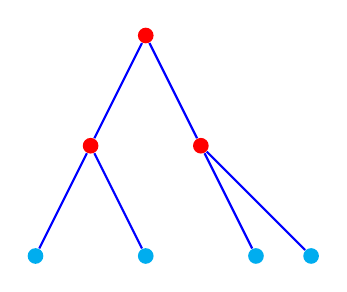
\begin{tikzpicture}[scale=0.7]
\node (n1) at (0,0) [circle, fill=red, inner sep=2pt]{};
\node (n2) at (-1,-2) [circle, fill=red, inner sep=2pt]{};
\node (n3) at (1,-2) [circle, fill=red, inner sep=2pt]{};
\node (n4) at (-2,-4) [circle, fill=cyan, inner sep=2pt]{};
\node (n5) at (0,-4) [circle, fill=cyan, inner sep=2pt]{};
\node (n6) at (2,-4) [circle, fill=cyan, inner sep=2pt]{};
\node (n7) at (3,-4) [circle, fill=cyan, inner sep=2pt]{};

\draw[blue, thick] (n1) -- (n2);
\draw[blue, thick] (n1) -- (n3);
\draw[blue, thick] (n2) -- (n4);
\draw[blue, thick] (n2) -- (n5);
\draw[blue, thick] (n3) -- (n6);
\draw[blue, thick] (n3) -- (n7);
\end{tikzpicture}
\end{center}

\begin{block}{Observation}
A tree on $m$ vertices has $m-1$ edges.
\end{block}

\end{frame}

\begin{frame}
\frametitle{Counting triangulations}

\begin{block}{Theorem}
The number of triangulations of a convex $(n + 2)$-gon by noncrossing diagonals is $C_n$.
\end{block}

\bigskip
Special case $n = 0$: one triangulation of a 2-gon.

\begin{block}{Proof idea: splitting a triangulation}
\begin{center}
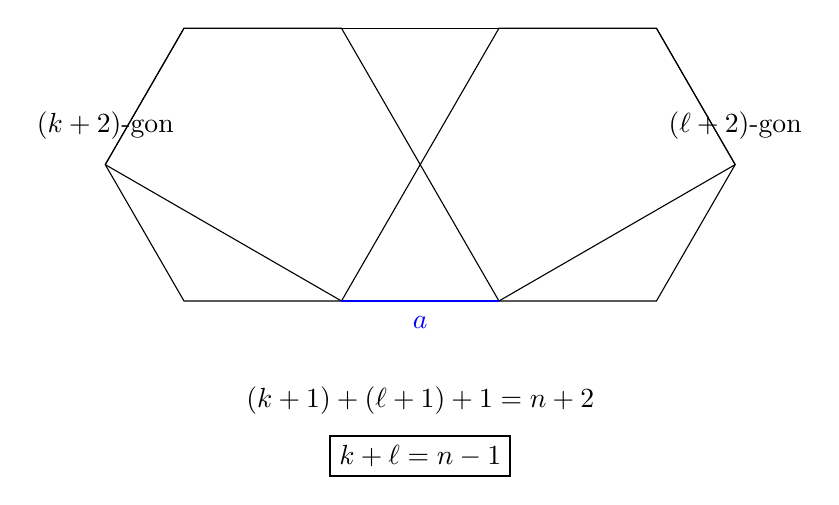
\begin{tikzpicture}
    \draw (0,0) -- (1,1.732) -- (3,1.732) -- (4,0) -- (3,-1.732) -- (1,-1.732) -- (0,0);
    \draw (0,0) -- (-1,1.732) -- (-3,1.732) -- (-4,0) -- (-3,-1.732) -- (-1,-1.732) -- (0,0);
    \draw (-4,0) -- (-3,1.732);
    \draw (-4,0) -- (-1,-1.732);
    \draw (4,0) -- (3,1.732);
    \draw (4,0) -- (1,-1.732);
    \draw (-3,1.732) -- (3,1.732);
    \draw (-1,-1.732) -- (1,-1.732);
    \draw[blue] (-1,-1.732) -- (1,-1.732);

    \node at (-4,0.5) {$(k+2)$-gon};
    \node at (4,0.5) {$(\ell+2)$-gon};
    \node[blue] at (0,-2) {$a$};
    \node at (0,-3) {$(k+1)+(\ell+1)+1=n+2$};
    \node[draw, thick] at (0,-3.7) {$k+\ell=n-1$};
\end{tikzpicture}
\end{center}
\end{block}

\end{frame}

\begin{frame}
    \frametitle{Counting triangulations}

    \begin{block}{Theorem}
        The number of triangulations of a convex $(n + 2)$-gon by noncrossing diagonals is $C_n$.
    \end{block}

    \begin{block}{Proof}
        Let $h_n$ denote the number of such triangulations. The splitting construction shows that the numbers $h_n$ satisfy the same recurrence
        \[
            h_n = \sum_{k+\ell=n-1} h_k h_\ell
        \]
        as the Catalan numbers. The claim follows by induction on $n$.

        \vspace{0.5cm}
        
        % Placeholder for the illustration
        % \begin{center}
        %     \begin{tikzpicture}
        %         \draw (0,0) -- (1,0) -- (1.5,0.8) -- (1,1.6) -- (0,1.6) -- (-0.5,0.8) -- cycle;
        %         \draw (0,0) -- (1,1.6);
        %         \draw (1,0) -- (0,1.6);
        %         \node at (0.5,-0.3) {$a$};
        %     \end{tikzpicture}
        % \end{center}

        (k+2)-gon \hspace{3cm} ($\ell$+2)-gon
        \vspace{0.5cm}

        \fbox{$k+\ell=n-1$}
    \end{block}
\end{frame}

\begin{frame}
\frametitle{Triangulations of a convex polygon by noncrossing diagonals}

\begin{center}
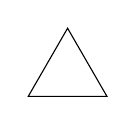
\begin{tikzpicture}
    \draw (0,0) -- (1,0) -- (0.5,0.866) -- cycle;
\end{tikzpicture}
\hspace{1cm}
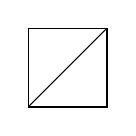
\begin{tikzpicture}
    \draw (0,0) -- (1,0) -- (1,1) -- (0,1) -- cycle;
    \draw (0,0) -- (1,1);
\end{tikzpicture}
\hspace{0.5cm}
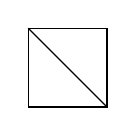
\begin{tikzpicture}
    \draw (0,0) -- (1,0) -- (1,1) -- (0,1) -- cycle;
    \draw (1,0) -- (0,1);
\end{tikzpicture}
\end{center}

\hrulefill

\begin{center}
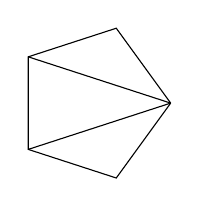
\begin{tikzpicture}
    \draw (0:1) \foreach \x in {72,144,...,360} { -- (\x:1) };
    \draw (0:1) -- (144:1);
    \draw (0:1) -- (216:1);
\end{tikzpicture}
\hspace{0.25cm}
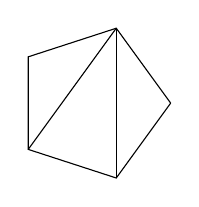
\begin{tikzpicture}
    \draw (0:1) \foreach \x in {72,144,...,360} { -- (\x:1) };
    \draw (72:1) -- (216:1);
    \draw (72:1) -- (288:1);
\end{tikzpicture}
\hspace{0.25cm}
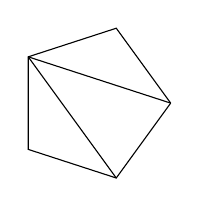
\begin{tikzpicture}
    \draw (0:1) \foreach \x in {72,144,...,360} { -- (\x:1) };
    \draw (144:1) -- (288:1);
    \draw (144:1) -- (360:1);
\end{tikzpicture}
\hspace{0.25cm}
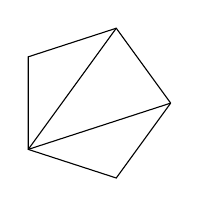
\begin{tikzpicture}
    \draw (0:1) \foreach \x in {72,144,...,360} { -- (\x:1) };
    \draw (216:1) -- (360:1);
    \draw (216:1) -- (72:1);
\end{tikzpicture}
\hspace{0.25cm}
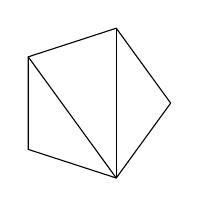
\begin{tikzpicture}
    \draw (0:1) \foreach \x in {72,144,...,360} { -- (\x:1) };
    \draw (288:1) -- (72:1);
    \draw (288:1) -- (144:1);
\end{tikzpicture}
\end{center}

\hrulefill

\begin{center}
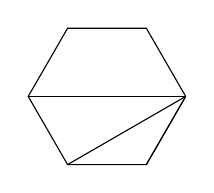
\begin{tikzpicture}
\draw (0:1) \foreach \x in {60,120,...,360} { -- (\x:1) };
\draw (0:1) -- (180:1);
\draw (0:1) -- (240:1);
\draw (0:1) -- (300:1);
\end{tikzpicture}
\hspace{0.25cm}
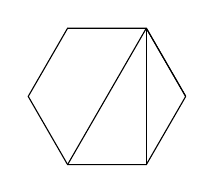
\begin{tikzpicture}
\draw (0:1) \foreach \x in {60,120,...,360} { -- (\x:1) };
\draw (60:1) -- (240:1);
\draw (60:1) -- (300:1);
\draw (60:1) -- (360:1);
\end{tikzpicture}
\hspace{0.25cm}
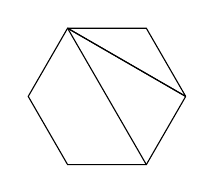
\begin{tikzpicture}
\draw (0:1) \foreach \x in {60,120,...,360} { -- (\x:1) };
\draw (120:1) -- (300:1);
\draw (120:1) -- (360:1);
\draw (120:1) -- (0:1);
\end{tikzpicture}
\hspace{0.25cm}
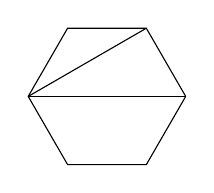
\begin{tikzpicture}
\draw (0:1) \foreach \x in {60,120,...,360} { -- (\x:1) };
\draw (180:1) -- (360:1);
\draw (180:1) -- (0:1);
\draw (180:1) -- (60:1);
\end{tikzpicture}
\hspace{0.25cm}
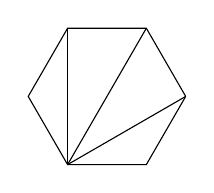
\begin{tikzpicture}
\draw (0:1) \foreach \x in {60,120,...,360} { -- (\x:1) };
\draw (240:1) -- (0:1);
\draw (240:1) -- (60:1);
\draw (240:1) -- (120:1);
\end{tikzpicture}
\end{center}

\begin{center}
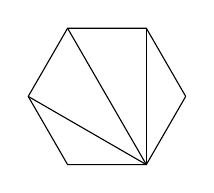
\begin{tikzpicture}
\draw (0:1) \foreach \x in {60,120,...,360} { -- (\x:1) };
\draw (300:1) -- (60:1);
\draw (300:1) -- (120:1);
\draw (300:1) -- (180:1);
\end{tikzpicture}
\hspace{0.25cm}
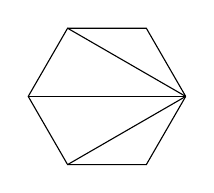
\begin{tikzpicture}
\draw (0:1) \foreach \x in {60,120,...,360} { -- (\x:1) };
\draw (360:1) -- (120:1);
\draw (360:1) -- (180:1);
\draw (360:1) -- (240:1);
\end{tikzpicture}
\hspace{0.25cm}
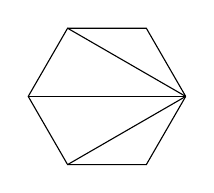
\begin{tikzpicture}
\draw (0:1) \foreach \x in {60,120,...,360} { -- (\x:1) };
\draw (0:1) -- (120:1);
\draw (0:1) -- (180:1);
\draw (0:1) -- (240:1);
\end{tikzpicture}
\hspace{0.25cm}
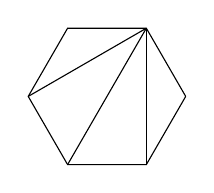
\begin{tikzpicture}
\draw (0:1) \foreach \x in {60,120,...,360} { -- (\x:1) };
\draw (60:1) -- (180:1);
\draw (60:1) -- (240:1);
\draw (60:1) -- (300:1);
\end{tikzpicture}
\hspace{0.25cm}
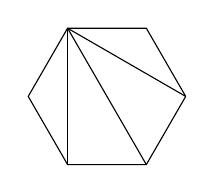
\begin{tikzpicture}
\draw (0:1) \foreach \x in {60,120,...,360} { -- (\x:1) };
\draw (120:1) -- (240:1);
\draw (120:1) -- (300:1);
\draw (120:1) -- (360:1);
\end{tikzpicture}
\end{center}

\begin{center}
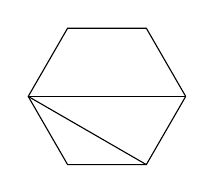
\begin{tikzpicture}
\draw (0:1) \foreach \x in {60,120,...,360} { -- (\x:1) };
\draw (180:1) -- (300:1);
\draw (180:1) -- (360:1);
\draw (180:1) -- (0:1);
\end{tikzpicture}
\hspace{0.25cm}
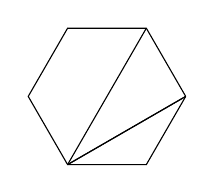
\begin{tikzpicture}
\draw (0:1) \foreach \x in {60,120,...,360} { -- (\x:1) };
\draw (240:1) -- (360:1);
\draw (240:1) -- (0:1);
\draw (240:1) -- (60:1);
\end{tikzpicture}
\hspace{0.25cm}
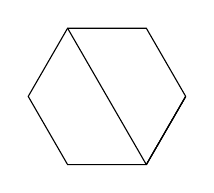
\begin{tikzpicture}
\draw (0:1) \foreach \x in {60,120,...,360} { -- (\x:1) };
\draw (300:1) -- (360:1);
\draw (300:1) -- (0:1);
\draw (300:1) -- (120:1);
\end{tikzpicture}
\hspace{0.25cm}
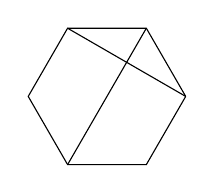
\begin{tikzpicture}
\draw (0:1) \foreach \x in {60,120,...,360} { -- (\x:1) };
\draw (0:1) -- (120:1);
\draw (60:1) -- (240:1);
\end{tikzpicture}
\hspace{0.25cm}
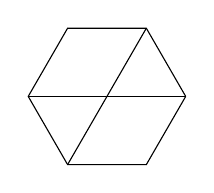
\begin{tikzpicture}
\draw (0:1) \foreach \x in {60,120,...,360} { -- (\x:1) };
\draw (0:1) -- (180:1);
\draw (60:1) -- (240:1);
\end{tikzpicture}
\end{center}

Triangulations that differ by rotation are viewed as distinct.

\end{frame}

\begin{frame}
\begin{center}
Math 465: Introduction to Combinatorics
\end{center}
\vspace{0.5cm}
\begin{center}
Andrew Sack
\end{center}
\vspace{0.5cm}
\hrulefill
\vspace{0.5cm}
\begin{center}
Homework \#4 will be due Monday evening.
\end{center}
\vspace{0.5cm}
\hrulefill
\vspace{0.5cm}
\begin{center}
Exam \#1 will be held in class on Thursday, February 27. \\
A ``crib sheet'' will be allowed. It can be 1 piece of paper up to \\
8.5"x11" and can be handwritten or typed.
\end{center}
\vspace{0.5cm}
\hrulefill
\vspace{0.5cm}
\begin{center}
These slides will be posted on Canvas.
\end{center}
\end{frame}

\begin{frame}
\frametitle{Counting complete binary trees}

\begin{block}{Theorem}
The number of complete binary trees with $n + 1$ leaves (equivalently, $n$ internal vertices) is $C_n$.
\end{block}

\begin{block}{Example: $n = 3$}
\begin{tabular}{ccccc}
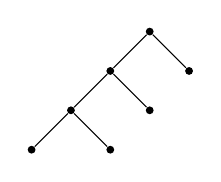
\begin{tikzpicture}[scale=0.5]
\node[circle, fill, inner sep=1pt] (r) at (0,3) {};
\node[circle, fill, inner sep=1pt] (a) at (-1,2) {};
\node[circle, fill, inner sep=1pt] (b) at (1,2) {};
\node[circle, fill, inner sep=1pt] (c) at (-2,1) {};
\node[circle, fill, inner sep=1pt] (d) at (0,1) {};
\node[circle, fill, inner sep=1pt] (e) at (-3,0) {};
\node[circle, fill, inner sep=1pt] (f) at (-1,0) {};

\draw (r) -- (a);
\draw (r) -- (b);
\draw (a) -- (c);
\draw (a) -- (d);
\draw (c) -- (e);
\draw (c) -- (f);
\end{tikzpicture}
&
\vline
&
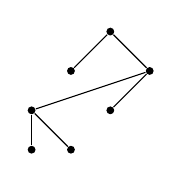
\begin{tikzpicture}[scale=0.5]
\node[circle, fill, inner sep=1pt] (r) at (0,3) {};
\node[circle, fill, inner sep=1pt] (a) at (-1,2) {};
\node[circle, fill, inner sep=1pt] (b) at (1,2) {};
\node[circle, fill, inner sep=1pt] (c) at (-2,1) {};
\node[circle, fill, inner sep=1pt] (d) at (0,1) {};
\node[circle, fill, inner sep=1pt] (e) at (-2,0) {};
\node[circle, fill, inner sep=1pt] (f) at (-1,0) {};

\draw (r) -- (a);
\draw (r) -- (b);
\draw (b) -- (c);
\draw (b) -- (d);
\draw (c) -- (e);
\draw (c) -- (f);
\end{tikzpicture}
&
\vline
&
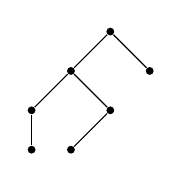
\begin{tikzpicture}[scale=0.5]
\node[circle, fill, inner sep=1pt] (r) at (0,3) {};
\node[circle, fill, inner sep=1pt] (a) at (-1,2) {};
\node[circle, fill, inner sep=1pt] (b) at (1,2) {};
\node[circle, fill, inner sep=1pt] (c) at (-2,1) {};
\node[circle, fill, inner sep=1pt] (d) at (0,1) {};
\node[circle, fill, inner sep=1pt] (e) at (-2,0) {};
\node[circle, fill, inner sep=1pt] (f) at (-1,0) {};

\draw (r) -- (a);
\draw (r) -- (b);
\draw (a) -- (c);
\draw (a) -- (d);
\draw (c) -- (e);
\draw (d) -- (f);
\end{tikzpicture}
\\
& & & & \\
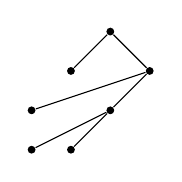
\begin{tikzpicture}[scale=0.5]
\node[circle, fill, inner sep=1pt] (r) at (0,3) {};
\node[circle, fill, inner sep=1pt] (a) at (-1,2) {};
\node[circle, fill, inner sep=1pt] (b) at (1,2) {};
\node[circle, fill, inner sep=1pt] (c) at (-2,1) {};
\node[circle, fill, inner sep=1pt] (d) at (0,1) {};
\node[circle, fill, inner sep=1pt] (e) at (-2,0) {};
\node[circle, fill, inner sep=1pt] (f) at (-1,0) {};

\draw (r) -- (a);
\draw (r) -- (b);
\draw (b) -- (c);
\draw (b) -- (d);
\draw (d) -- (e);
\draw (d) -- (f);
\end{tikzpicture}
&
\vline
&
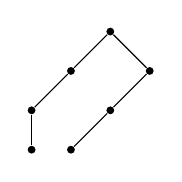
\begin{tikzpicture}[scale=0.5]
\node[circle, fill, inner sep=1pt] (r) at (0,3) {};
\node[circle, fill, inner sep=1pt] (a) at (-1,2) {};
\node[circle, fill, inner sep=1pt] (b) at (1,2) {};
\node[circle, fill, inner sep=1pt] (c) at (-2,1) {};
\node[circle, fill, inner sep=1pt] (d) at (0,1) {};
\node[circle, fill, inner sep=1pt] (e) at (-2,0) {};
\node[circle, fill, inner sep=1pt] (f) at (-1,0) {};

\draw (r) -- (a);
\draw (r) -- (b);
\draw (a) -- (c);
\draw (b) -- (d);
\draw (c) -- (e);
\draw (d) -- (f);
\end{tikzpicture}
\end{tabular}

\end{block}

\end{frame}

\begin{frame}
\frametitle{Complete binary trees}

\begin{block}{Definition}
A \textcolor{blue}{complete binary tree} is an ordered rooted tree in which each
internal vertex has exactly two children (designated \textcolor{blue}{left} and \textcolor{blue}{right}).

\begin{center}
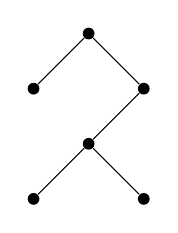
\begin{tikzpicture}[scale=0.7]
\node[circle, fill, inner sep=1.5pt] (root) at (0,2) {};
\node[circle, fill, inner sep=1.5pt] (a) at (-1,1) {};
\node[circle, fill, inner sep=1.5pt] (b) at (1,1) {};
\node[circle, fill, inner sep=1.5pt] (c) at (0,0) {};
\node[circle, fill, inner sep=1.5pt] (d) at (-1,-1) {};
\node[circle, fill, inner sep=1.5pt] (e) at (1,-1) {};

\draw (root) -- (a);
\draw (root) -- (b);
\draw (b) -- (c);
\draw (c) -- (d);
\draw (c) -- (e);
\end{tikzpicture}
\end{center}
\end{block}

\begin{block}{Lemma}
A complete binary tree with $n$ internal vertices has $n + 1$ leaves.
\end{block}

\begin{block}{Proof}
Induction on $n$. Find two sibling leaves, then remove them together
with the two edges that connect to them. Both the number of leaves
and the number of internal vertices decrease by 1.
\end{block}

\end{frame}

\begin{frame}
\frametitle{Counting complete binary trees}

\begin{block}{Theorem}
The number of complete binary trees with $n + 1$ leaves (equivalently, $n$ internal vertices) is $C_n$.
\end{block}

\begin{block}{Proof}
A complete binary tree with $n \geq 1$ internal vertices splits into the left and right (complete binary) subtrees with $k$ and $\ell$ internal vertices, respectively, with $k + \ell = n - 1$:

\begin{center}
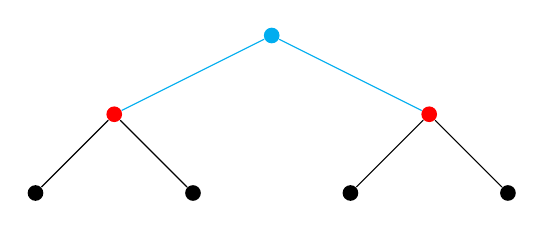
\begin{tikzpicture}
  \node[circle, fill=cyan, inner sep=2pt] (root) at (0,0) {};
  \node[circle, fill=red, inner sep=2pt] (left) at (-2,-1) {};
  \node[circle, fill=red, inner sep=2pt] (right) at (2,-1) {};
  \node[circle, fill=black, inner sep=2pt] (left_left) at (-3,-2) {};
  \node[circle, fill=black, inner sep=2pt] (left_right) at (-1,-2) {};
  \node[circle, fill=black, inner sep=2pt] (right_left) at (1,-2) {};
  \node[circle, fill=black, inner sep=2pt] (right_right) at (3,-2) {};

  \draw[cyan] (root) -- (left);
  \draw[cyan] (root) -- (right);
  \draw (left) -- (left_left);
  \draw (left) -- (left_right);
  \draw (right) -- (right_left);
  \draw (right) -- (right_right);
\end{tikzpicture}
\end{center}

Hence the numbers $h_n$ counting such trees satisfy $h_n = \sum_{k+\ell=n-1} h_k h_\ell$.

The claim follows by induction on $n$.
\end{block}

\end{frame}

\begin{frame}
\frametitle{Complete binary trees and triangulations}

\begin{block}{Proposition}
Complete rooted binary trees with $n+1$ leaves are in bijection with triangulations of a convex $(n+2)$-gon by noncrossing diagonals.
\end{block}

\begin{center}
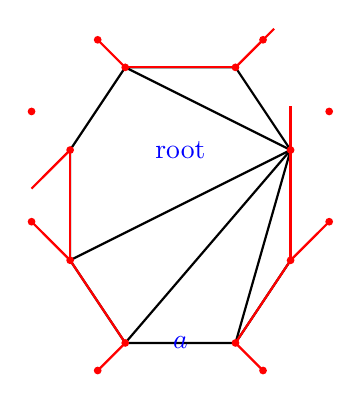
\begin{tikzpicture}[scale=0.7]
    % Draw the octagon
    \coordinate (A) at (0,0);
    \coordinate (B) at (2,0);
    \coordinate (C) at (3,1.5);
    \coordinate (D) at (3,3.5);
    \coordinate (E) at (2,5);
    \coordinate (F) at (0,5);
    \coordinate (G) at (-1,3.5);
    \coordinate (H) at (-1,1.5);

    \draw[thick] (A) -- (B) -- (C) -- (D) -- (E) -- (F) -- (G) -- (H) -- cycle;

    % Draw diagonals
    \draw[thick] (A) -- (D);
    \draw[thick] (D) -- (F);
    \draw[thick] (B) -- (D);
    \draw[thick] (D) -- (H);

    % Draw the tree
    \draw[red, thick] (A) -- +(-0.5,-0.5);
    \draw[red, thick] (B) -- +(0.5,-0.5);
    \draw[red, thick] (C) -- +(0.5,0.5);
    \draw[red, thick] (D) -- +(0,0.8);
    \draw[red, thick] (E) -- +(0.5,0.5);
    \draw[red, thick] (F) -- +(-0.5,0.5);
    \draw[red, thick] (G) -- +(-0.5,-0.5);
    \draw[red, thick] (H) -- +(-0.5,0.5);

    \draw[red, thick] (A) -- (H);
    \draw[red, thick] (H) -- +(-0.7,0.7);
    \draw[red, thick] (H) -- (G);
    \draw[red, thick] (G) -- +(-0.7,-0.7);
    \draw[red, thick] (F) -- (E);
    \draw[red, thick] (E) -- +(0.7,0.7);
    \draw[red, thick] (D) -- (C);
    \draw[red, thick] (C) -- +(0.7,0.7);
    \draw[red, thick] (B) -- (C);

    \node[blue] at (1,0) {$a$};
    \node[blue] at (1,3.5) {root};

    % Draw dots at vertices
    \foreach \point in {A,B,C,D,E,F,G,H}
        \fill[red] (\point) circle (2pt);
    \fill[red] (-1.7,2.2) circle (2pt);
    \fill[red] (3.7,2.2) circle (2pt);
    \fill[red] (3.7,4.2) circle (2pt);
    \fill[red] (-1.7,4.2) circle (2pt);
    \fill[red] (-0.5,-0.5) circle (2pt);
    \fill[red] (2.5,-0.5) circle (2pt);
    \fill[red] (2.5,5.5) circle (2pt);
    \fill[red] (-0.5,5.5) circle (2pt);
\end{tikzpicture}
\end{center}

\end{frame}

\begin{frame}
Exercise

Give a direct bijection between rooted ordered trees and complete binary trees.
\end{frame}

\begin{frame}
Exercise

A \textit{binary tree} is a rooted tree where each vertex can have a left child, a right child, both, or neither. Give a bijection between binary trees and complete binary trees.
\end{frame}

\begin{frame}
Exercise

Show that the Catalan numbers count the number of ways to fill a $2 \times n$ checkerboard with the numbers $1, \dots, n$ such that the numbers increase within each row and column.
\end{frame}

\begin{frame}
Exercise

Prove that $\sum_{k=0}^{n} C_{2k} C_{2(n-k)} = 4^n C_n$.

(This is very hard if you don't use generating functions.)
\end{frame}

\begin{frame}
    \frametitle{Bracketings vs. ballot sequences}

    We shall construct a bijection between the bracketings of $n+1$ letters and the ballot sequences of length $2n$.

    Let us add an extra pair of parentheses on the outside:
    
    $(((ab)c)d) \quad ((ab)(cd)) \quad ((a(bc))d) \quad (a((bc)d)) \quad (a(b(cd)))$

    Now each bracketing has $n$ opening and $n$ closing parentheses.

    These $2n$ parentheses form a ballot sequence.

    However this construction does \textbf{not} yield a desired bijection.

    \bigskip
    \centering
    \begin{center}
    \setlength\fboxsep{3pt}
        \colorbox{gray!30}{\begin{minipage}{0.9\textwidth}
            \textbf{Exercise}

            Prove that the following construction yields a bijection between bracketings of $n + 1$ letters and ballot sequences of length $2n$:

            Remove all closing parentheses. Replace each opening parenthesis with a $\boxed{+}$. Replace each letter, except for the last one, with a $\boxed{-}$.

            \bigskip

            $(((ab)c)d) \quad ((ab)(cd)) \quad ((a(bc))d) \quad (a((bc)d)) \quad (a(b(cd)))$
            
            $+\!+\!+\!-\!-\!-\!-\quad +\!+\!-\!-\!+\!-\quad +\!+\!-\!+\!-\!-\!-\quad +\!-\!+\!+\!-\!-\!-\quad +\!-\!+\!-\!+\!-\!-$
        \end{minipage}}
    \end{center}
\end{frame}

\begin{frame}
\frametitle{Bracketings}

\begin{block}{Theorem}
The number of syntactically correct bracketings of a given sequence
of $n + 1$ letters is $C_n$.
\end{block}

\begin{block}{Example: $n = 3$}
$((ab)c)d \quad (ab)(cd) \quad (a(bc))d \quad a((bc)d) \quad a(b(cd))$
\end{block}

\begin{block}{Proof}
The \textcolor{blue}{parse tree} construction provides a bijection between bracketings
of $n + 1$ letters and complete binary trees with $n + 1$ leaves.

\begin{tikzpicture}
\node[circle, fill, inner sep=1pt] (root) at (0,0) {};
\node[circle, fill, inner sep=1pt] (a) at (-1,-1) {};
\node[circle, fill, inner sep=1pt] (b) at (1,-1) {};
\node[circle, fill, inner sep=1pt] (c) at (0,-2) {};
\node[circle, fill, inner sep=1pt] (d) at (-1,-3) {};
\node[circle, fill, inner sep=1pt] (e) at (1,-3) {};

\draw (root) -- (a);
\draw (root) -- (b);
\draw (b) -- (c);
\draw (b) -- (e);
\draw (c) -- (d);

\node[anchor=east] at (a) {$a$};
\node[anchor=east] at (d) {$b$};
\node[anchor=west] at (e) {$c$};
\node[anchor=west] at (c) {$d$};

\node at (4,-2) {$a((bc)d)$};
\end{tikzpicture}
\end{block}

\end{frame}

\begin{frame}
\frametitle{Bijections between Catalan families}

We constructed bijections between the following families of
combinatorial objects counted by the Catalan numbers $C_n$:
\vspace{0.5cm}

\begin{minipage}{0.45\textwidth}
\begin{center}
\fbox{
\begin{tabular}{c}
bracketings \\
of $n + 1$ letters
\end{tabular}
}
\vspace{0.2cm}

$\updownarrow \hspace{-0.1cm} \downarrow$
\vspace{0.2cm}

\fbox{
\begin{tabular}{c}
complete binary trees \\
with $n + 1$ leaves
\end{tabular}
}
\vspace{0.2cm}

$\updownarrow \hspace{-0.1cm} \downarrow$
\vspace{0.2cm}

\fbox{
\begin{tabular}{c}
triangulations of an $(n + 2)$-gon \\
by noncrossing diagonals
\end{tabular}
}
\end{center}
\end{minipage}
\hfill
\begin{minipage}{0.45\textwidth}
\begin{center}
\fbox{
\begin{tabular}{c}
circular arrangements of \\
$n + 1$ $\boxed{+}$'s and $n$ $\boxed{-}$'s
\end{tabular}
}
\vspace{0.2cm}

$\updownarrow \hspace{-0.1cm} \downarrow$
\vspace{0.2cm}

\fbox{
\begin{tabular}{c}
ballot sequences \\
of length $2n$
\end{tabular}
}
\vspace{0.2cm}

$\updownarrow \hspace{-0.1cm} \downarrow$
\vspace{0.2cm}

\fbox{
\begin{tabular}{c}
ordered rooted trees on \\
$n + 1$ unlabeled vertices
\end{tabular}
}
\end{center}
\end{minipage}

\vspace{0.5cm}

Is there a bijection linking the families on the left and on the right?

\end{frame}
\end{document}